%___________________________ Q 4.6 ______________________________
\subsection{Comment on effect of the inclusion of a pre-filter. (2 pts)}
\vspace{10pt}

%%Write your answer here

Pre-filtering can play a vital role in shaping the reference signal before it enters the feedback loop by adjusting the input signal to compensate any new dynamics introduced by the controller or the plant. 

One of filters present in our system was an integrator, which was used to eliminate the steady-state error and push the system toward the desired output, this was particularly useful since the dead zone of the motor and gearbox introduced a non modulated error, that mean for a small value of the actuaction signal, was noticed to be around 0.2V,  the system would not move as we see in figure \ref{fig: Steady state error}. Something important to note in our integral is we have saturation limits, this was done to avoid any type of integral windup that could have happened. These saturation limits in our system were set to -2.5V and 2.5V, since the with the value of R choosen the maximum optimal control signal that we seen was around 5V, so we decided in a saturation of 2.5V since it would make sure the integral could never overwrite the maximum optimal control signal.  

\begin{figure}
    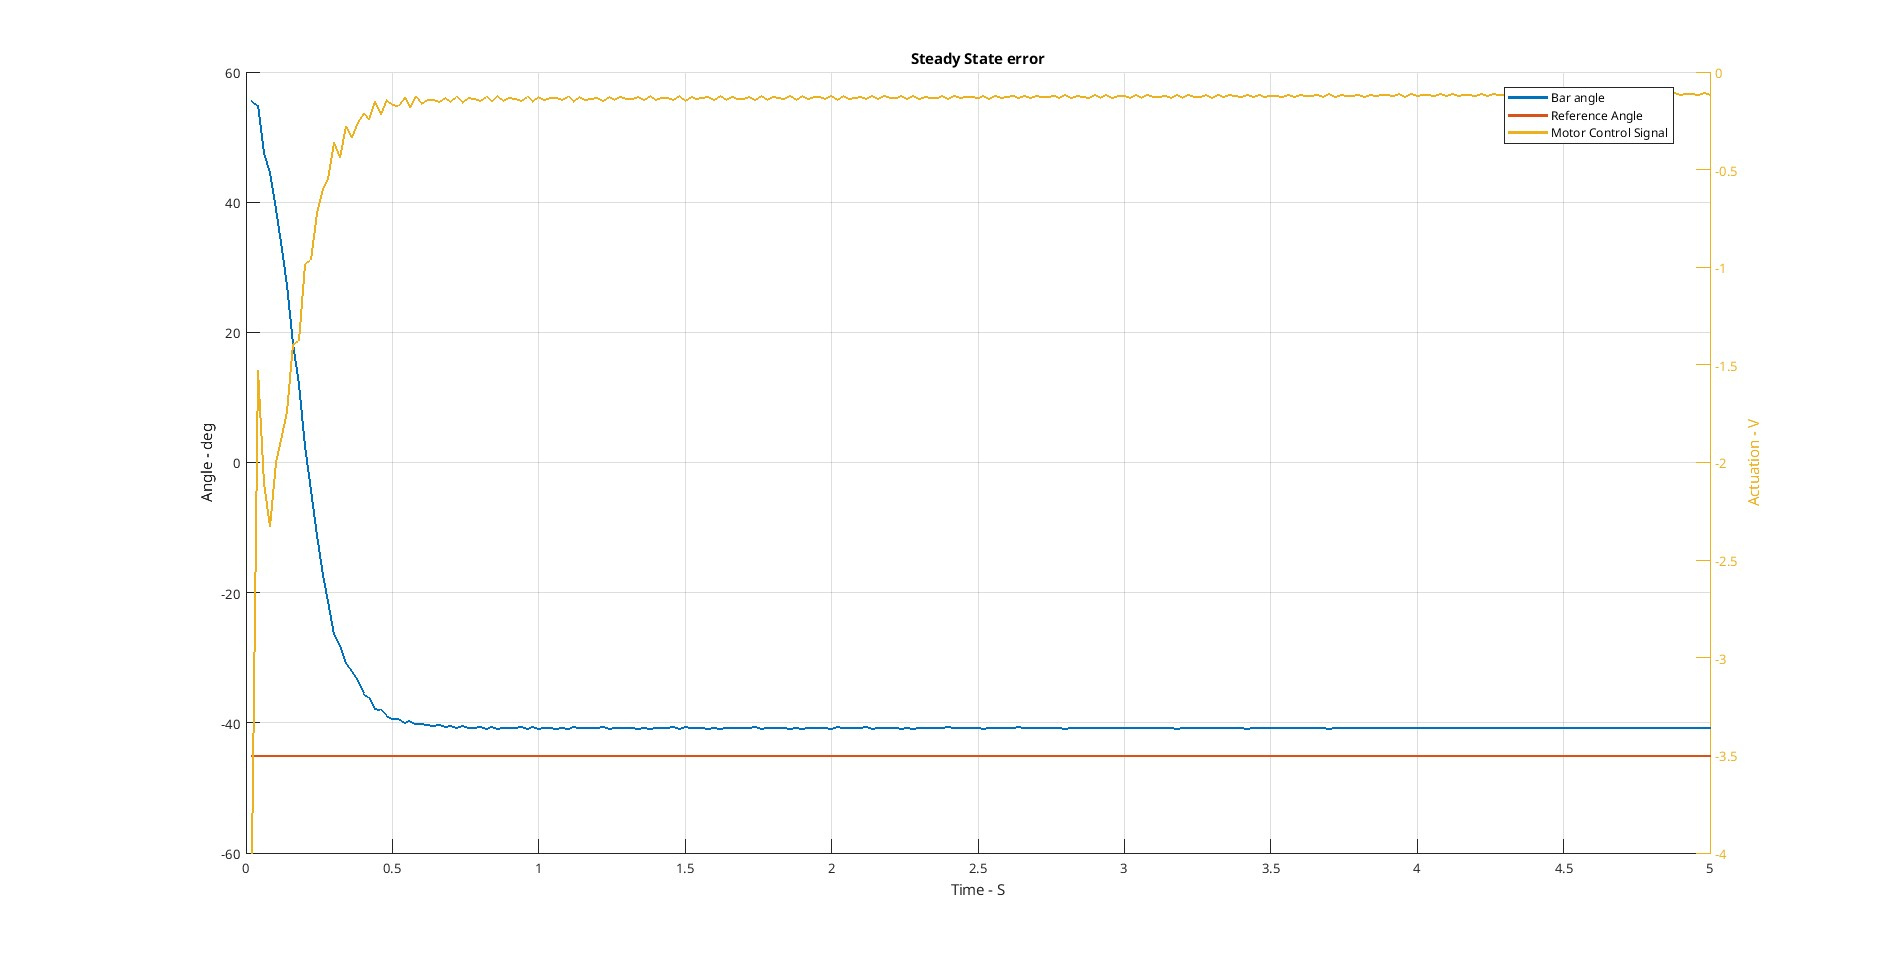
\includegraphics[width=0.7\textwidth]{Figs/steadyStateError.jpg}
    \caption{steady State Error}
    \label{fig: Steady state error}
\end{figure}

Another pre-filter present in our system was the kalman filter, and this is a rather important was, since as discussed earlier allows us to estimate the state of the system from the output, the control action and the model. 